\section{Bubonic plague}

\yp{} was identified in 1894 by Alexandre Yersin, during the epidemic then
running in Hong Kong. It was later attributed --- and only recently confirmed
with ancient genomic data --- to a series of pandemics which killed a huge
proportion of the European population and went on to shape the course of
western cultural development.

The first of these opened with the Justinianic plague of 541, and its
recurrences ran on into the eighth century. The second and most dramatic began
in the 1340s and may have killed as much as half of the European population
\cite{belich2022world}, a figure reaching above 80\% in some urban centres.
Successive waves of infection followed, and the continent did not fully emerge
from the plight until as late as the seventeenth century, with the fire of
London in 1666 often taken as the watershed moment.

\begin{figure}[tb]
\centering
% The panel widths are in the ratio of the two aspect ratios (1.4022 and
% 1.3444), so filling each box gives both images the same height and the pair
% reads as a diptych. They sum to 0.977, leaving a 10pt gutter to \hfill.
\begin{subfigure}[b]{0.4990\textwidth}
\centering
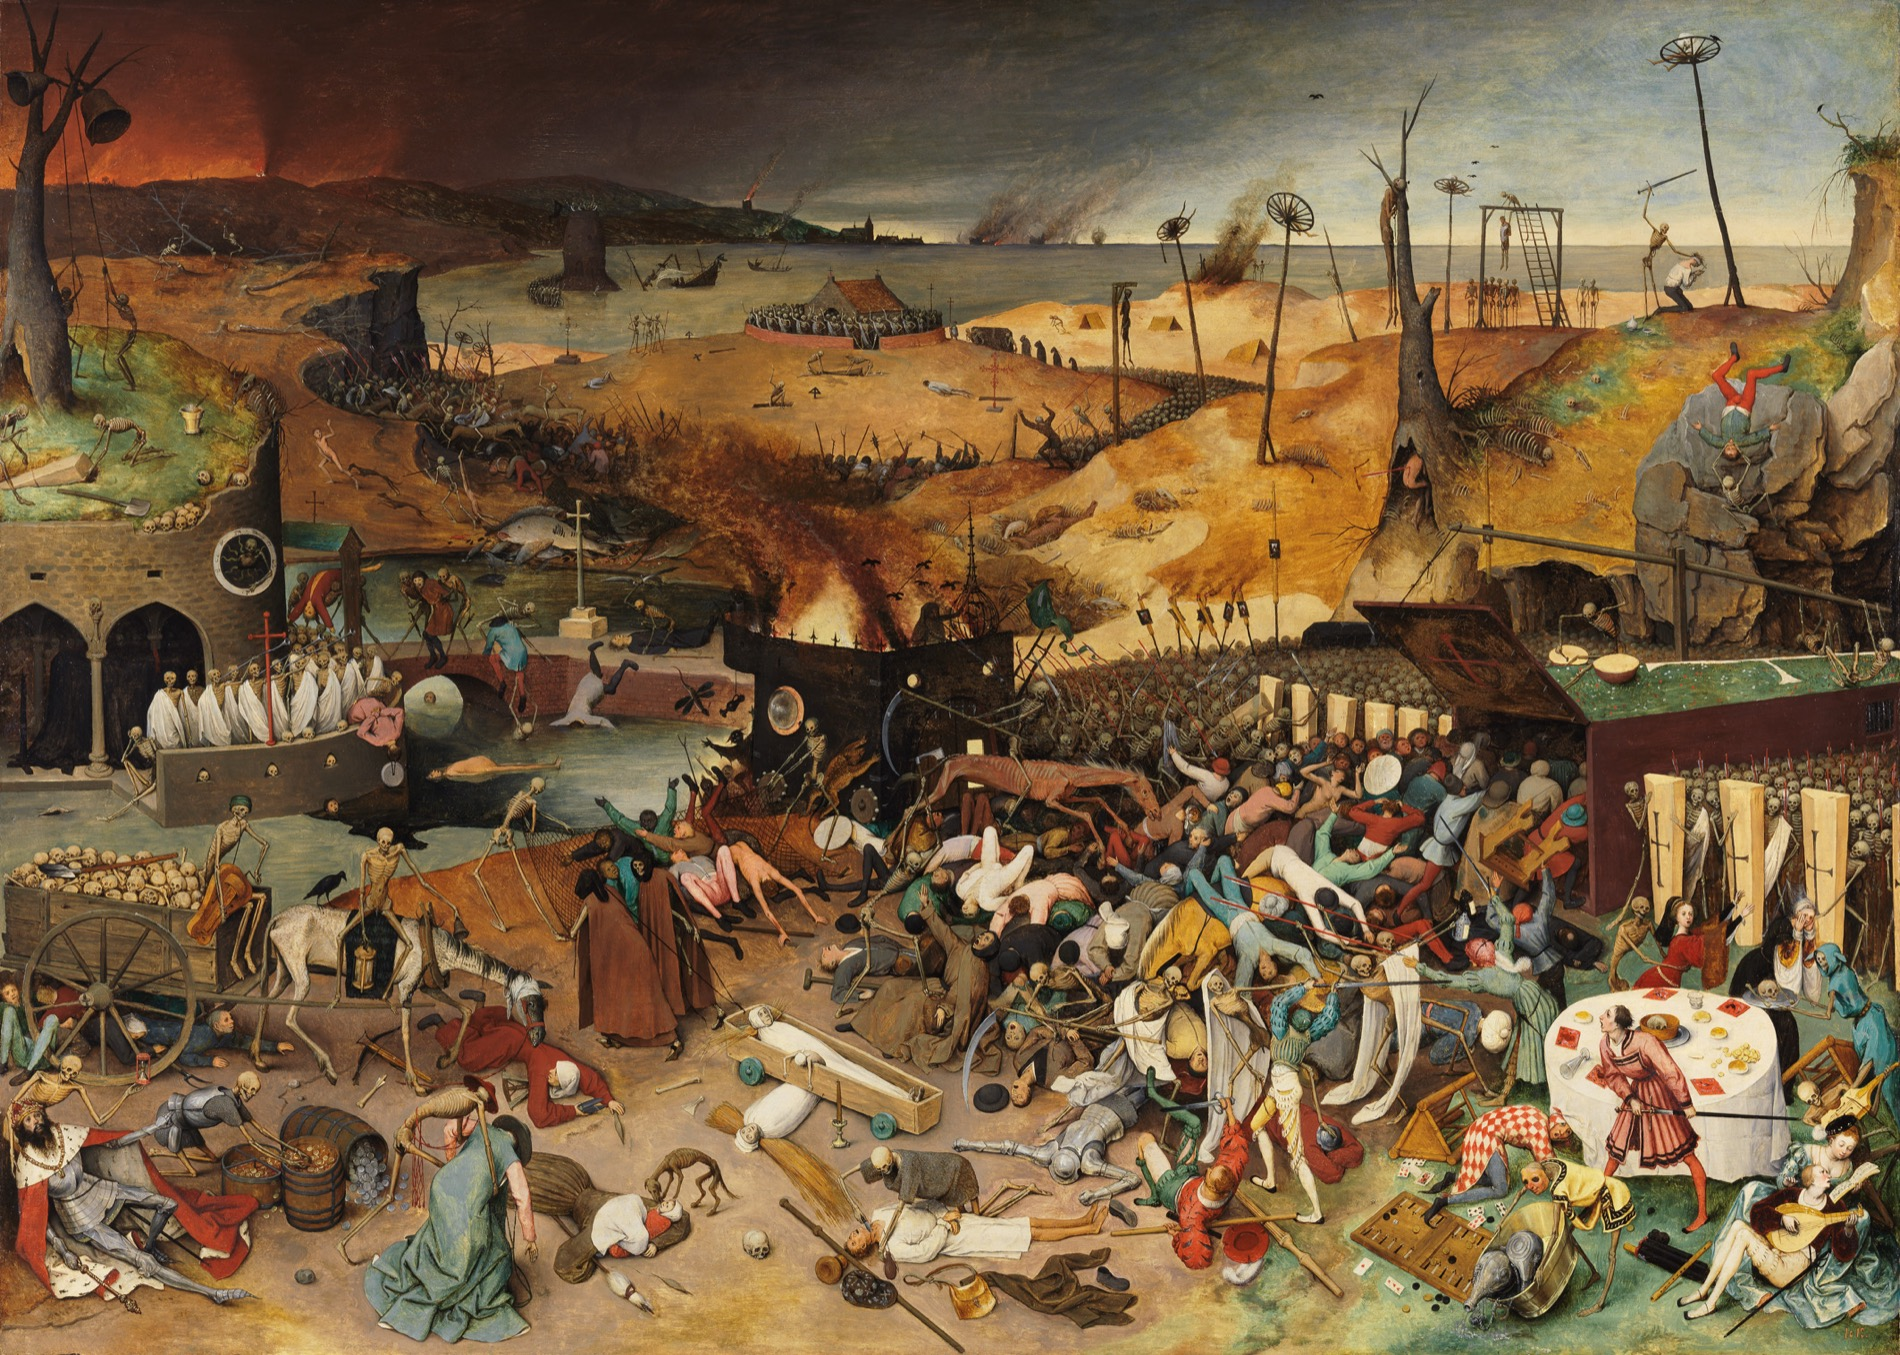
\includegraphics[width=\linewidth]{figures/fig_triumph/bruegel_triumph}
\caption*{(a) Bruegel, \textit{The Triumph of Death}.}
\end{subfigure}%
\hfill
\begin{subfigure}[b]{0.4784\textwidth}
\centering
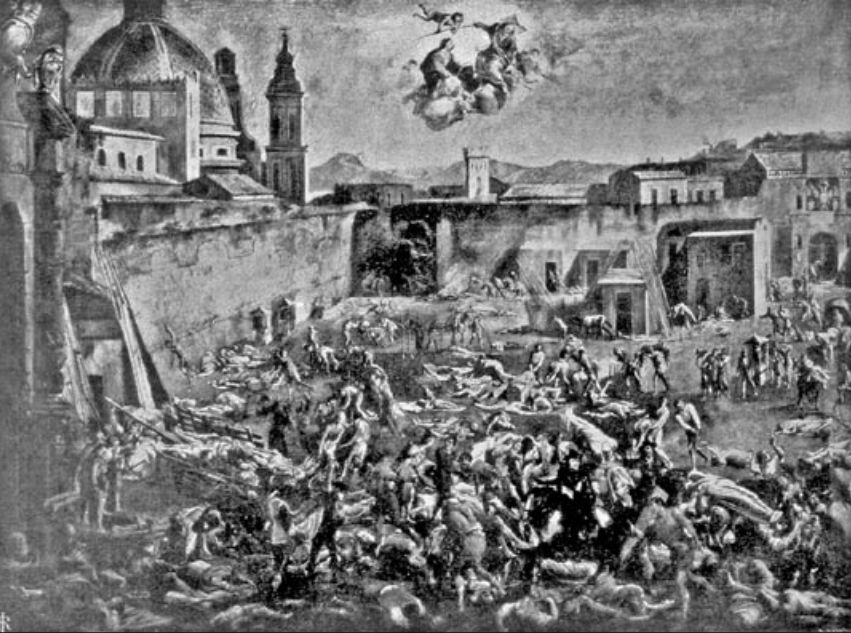
\includegraphics[width=\linewidth]{figures/fig_plague_naples/spadaro_naples_1656}
\caption*{(b) Spadaro, \textit{Piazza Mercatello}.}
\end{subfigure}
\caption{Plague in the European imagination, in allegory and in reportage.
(a)~\textit{The Triumph of Death}, Pieter Bruegel the Elder, c.~1562 (Museo del
Prado, Madrid). An army of skeletons lays waste to a landscape in which every
human occupation is interrupted at once; in the lower right the card game, the
banquet and the lute player have not yet noticed. The painting is an allegory
of death in general rather than a record of an epidemic, but it was made in a
Europe that had lived with recurrent plague for two centuries.
(b)~\textit{Piazza Mercatello a Napoli durante la peste del 1656}, Domenico
Gargiulo, called Micco Spadaro (Museo Nazionale di San Martino, Naples). Here
there is no allegory: a single square in a real city during a real outbreak,
the dead laid out in rows and the living still at work among them. Naples is
thought to have lost something close to half its population in that year.}
\label{fig:plague_art}
\end{figure}

There were likely earlier \yp{} epidemics reaching far back into history,
beyond the scope of accurate written account and recorded only in legend and
myth. The organism is now thought to have emerged from its evolutionary
antecedent, \textit{Yersinia pseudotuberculosis}, some six thousand years ago,
during what would have been a period of human population expansion driven by
the development of agriculture. One may hypothesise that it was this excess
supply of replicative means which provided the raw material for evolution,
facilitating a shift of phenotype over the saddle and into a new local optimum
--- the niche pathogenesis observed in \yp{} today. Whether rates of
diversification really do move with the supply of room is a question taken up,
in a quite different setting, by \mextref{var:ch:rates}{Chapter~9}.

